\documentclass[11pt]{article}
\usepackage{amsmath,amssymb,amsthm}
\usepackage{graphicx}
\usepackage{booktabs}
\usepackage[table]{xcolor}
\usepackage{float}
\usepackage{hyperref}
\usepackage{natbib}

\title{Internet Appendix: Detailed Options Data Cleaning and Portfolio Construction Procedures}
\author{}
\date{}

\begin{document}

\maketitle

\section{SPX Options Data Cleaning and Portfolio Construction}

This appendix provides comprehensive technical details on the data cleaning and portfolio construction procedures used for the SPX options dataset in our study. We follow the methodology of \citet{Constantinides2013} (``CJS'') with the highest practical fidelity.

\subsection{Phase 1a: Data Filtration in \citet{Constantinides2013}}

In order to minimize possible quoting errors, CJS filtered the raw options data through three levels of filters. The filters are applied to the trade-in (buy) side to ensure the portfolios are buying into reliable quotes. When positions are exited, if there is no quote in the filtered data, the raw data is searched. These filters are detailed in \textit{Appendix B} of CJS.



\subsubsection{Level 1 Filters}
\begin{itemize}
  \item \textbf{Identical Filter:} Retain only one instance of quotes with the same \textit{option type}, \textit{strike price}, \textit{expiration date/maturity}, and \textit{price}.
  \item \textbf{Identical Except Price Filter:} For sets of quotes with identical terms (\textit{type}, \textit{strike}, and \textit{maturity}) but different prices, keep the quote whose \textit{T-bill-based implied volatility} is closest to that of its \textit{moneyness neighbors}, and delete the others.
  \item \textbf{Bid = 0 Filter:} Drop quotes with a \textit{bid price} of zero, thereby avoiding low-valued options. Also, a zero bid may indicate censoring as negative bids cannot be recorded.
  \item \textbf{Volume = 0 Filter:} Drop quotes with zero volume. Appendix B of CJS does not explicitly detail this filter, but we list it here for completeness since it is included in Table B.1 (Filters) of CJS. However, given that \textit{Appendix B} of \citet{Constantinides2013} did not describe this filter, we assume its inclusion in Table B.1 (Filter) of CJS was an error, and we have not implemented this filter in our replication.
\end{itemize}


\subsubsection{Level 2 Filters}
\begin{itemize}
  \item \textbf{Days to Maturity Filter:} Drop options with fewer than seven or more than 180 calendar days to expiration.
  \item \textbf{Implied Volatility Filter:} Remove all option quotes with implied volatilities lower than 5\% or higher than 100\%, computed using T-bill interest rates.
  \item \textbf{Moneyness Filter:} Remove all option quotes with moneyness (the ratio of strike price to index price) below 0.8 or above 1.2. These options have little value beyond their intrinsic value and are also very thinly traded.
  \item \textbf{Implied Interest Rate Filter:} Compute implied volatilities using T-bill interest rates from the Federal Reserve's H.15 release, assigning the closest available rate to each observation. Since T-bill rates may not be relevant for short maturities, we also compute a put-call parity-implied interest rate by imposing put-call parity on put-call pairs and adjusting the interest rate. We remove pairs with negative implied interest rates and assign the median-implied rate to all quotes of the same maturity and moneyness between 0.95 and 1.05, interpolating as needed.
  \item \textbf{Unable to Compute IV Filter:} Remove quotes that imply negative time value.
\end{itemize}

\subsubsection{Level 3 Filters}
\begin{itemize}
  \item \textbf{IV Filter:} The IV filter removes volatility outliers to reduce the prevalence of apparent butterfly arbitrage. This involves dropping calls and puts that have the same expiration date and strike price, but have anomalous prices due to extreme implied volatility values. For each date and maturity, we fit a quadratic curve to the implied volatility of puts and calls (separately) through the observed log implied volatilities.
  \item \textbf{Put-Call Parity Filter:} The puts and calls need to be matched up based on trading date, expiry date, and option type. We then calculate the put-call parity implied interest rate, and filter out outliers based on the standard deviation of the relative distance between the interest rate implied by put-call parity, and the calculated daily median 3-month T-bill rate from the pulled data.
\end{itemize}


\begin{figure}[H]
  \centering
  \begin{tabular}{@{}c@{}}
    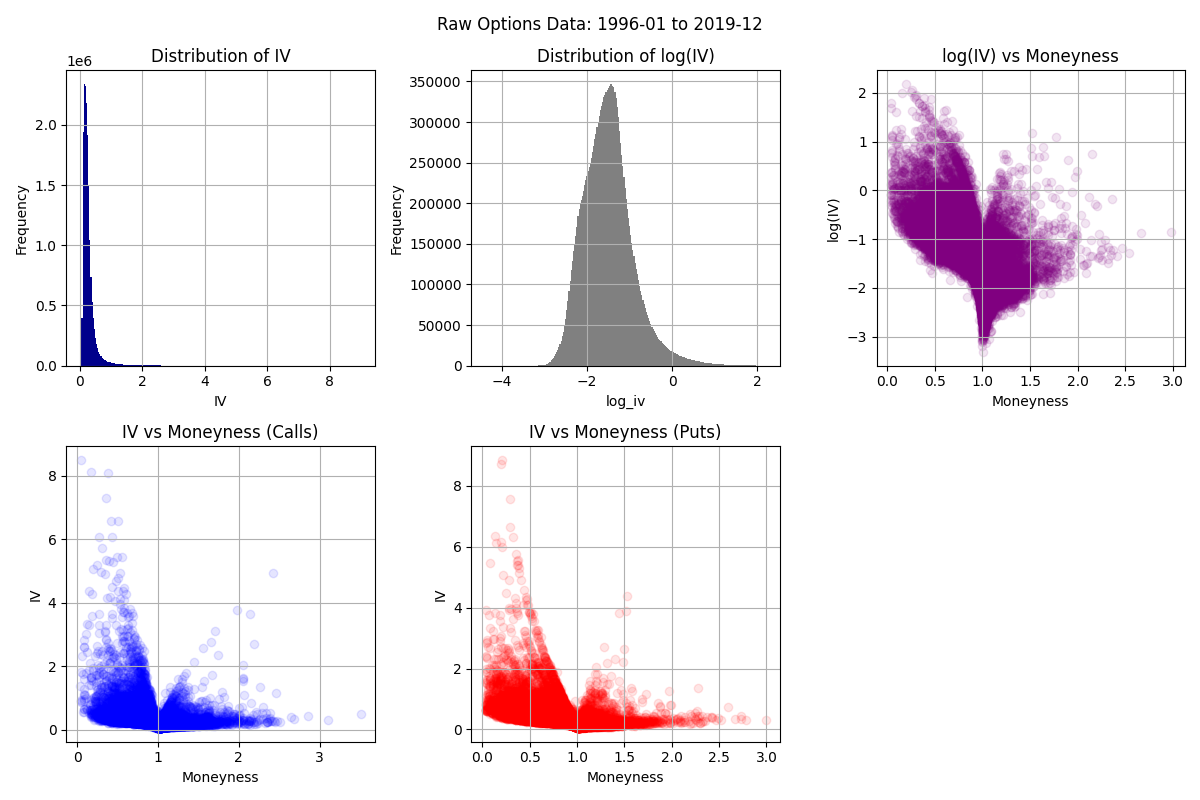
\includegraphics[width=\linewidth,height=0.666\linewidth]{../docs_src/RAW_1996-01_2019-12_iv.png}
  \end{tabular}
  \caption{Some visualizations of the raw SPX options data, prior to application of any filters. Each dot / point on these charts represents a single option in the raw data. Note that the time dimension is not shown, so this is a cross-sectional view of all options in the dataset.}
  \label{fig:raw_spx_options_data}
\end{figure}

\begin{figure}[H]
  \centering
  \begin{tabular}{@{}c@{}}
    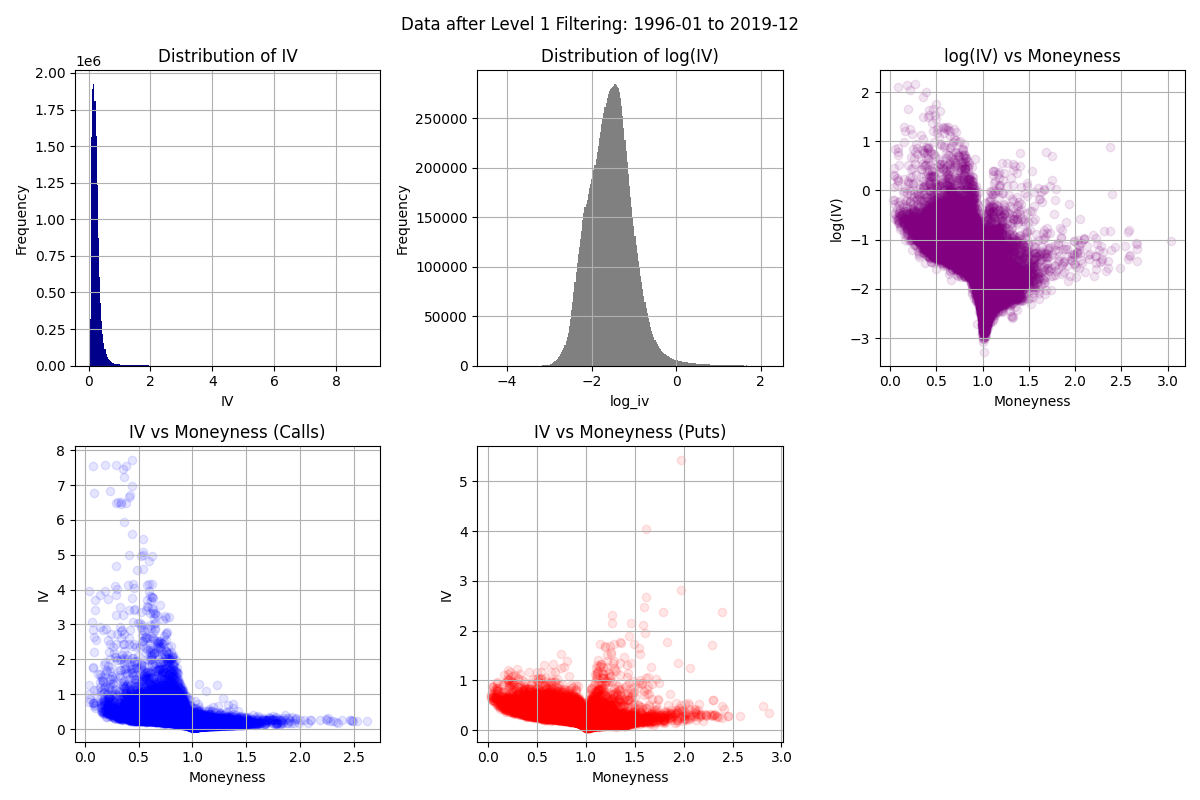
\includegraphics[width=\linewidth,height=0.666\linewidth]{../docs_src/L1_1996-01_2019-12_iv.png}
  \end{tabular}
  \caption{SPX options remaining after application of Level 1 filters. Notice reduction in outliers and cleaner distribution of volatility vs moneyness.}
  \label{fig:l1_spx_options_data}
\end{figure}


\begin{figure}[H]
  \centering
  \begin{tabular}{@{}c@{}}
    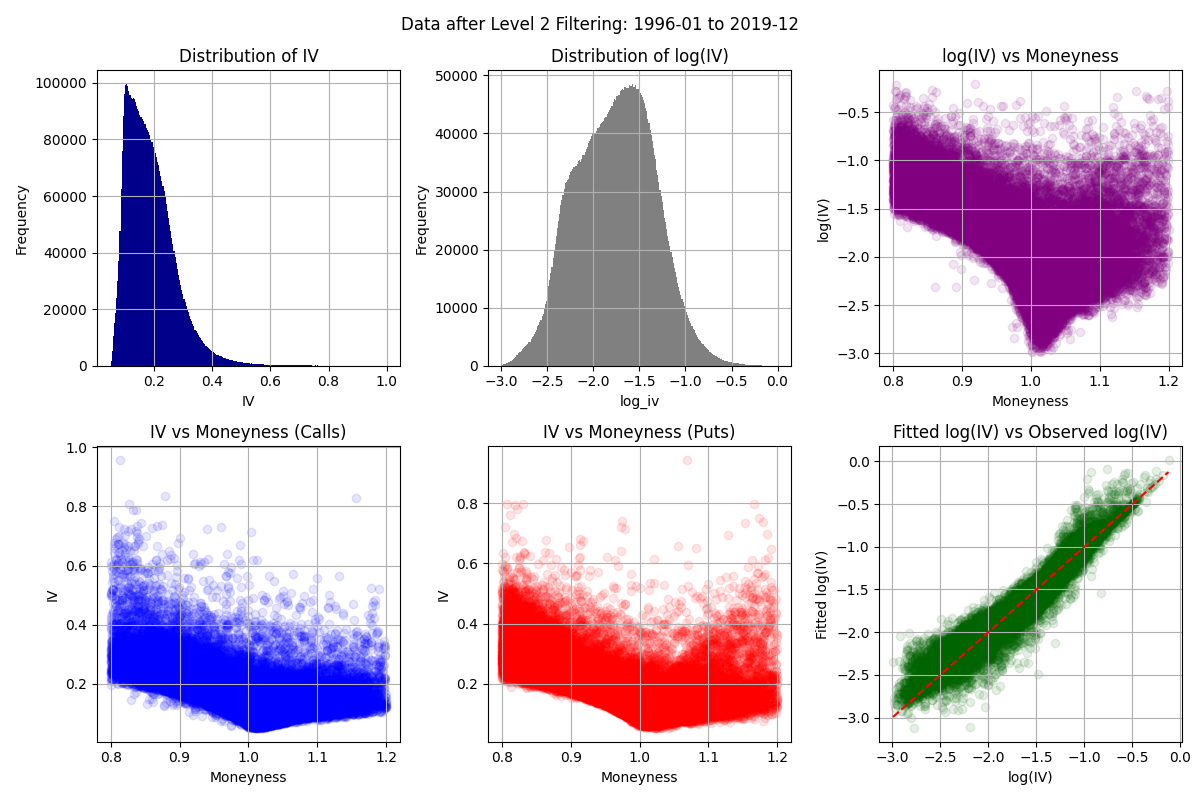
\includegraphics[width=\linewidth,height=0.666\linewidth]{../docs_src/L2_1996-01_2019-12_iv.png}
  \end{tabular}
  \caption{SPX options remaining after Level 2 filters.}
  \label{fig:l2_spx_options_data}
\end{figure}


\begin{figure}[H]
  \centering
  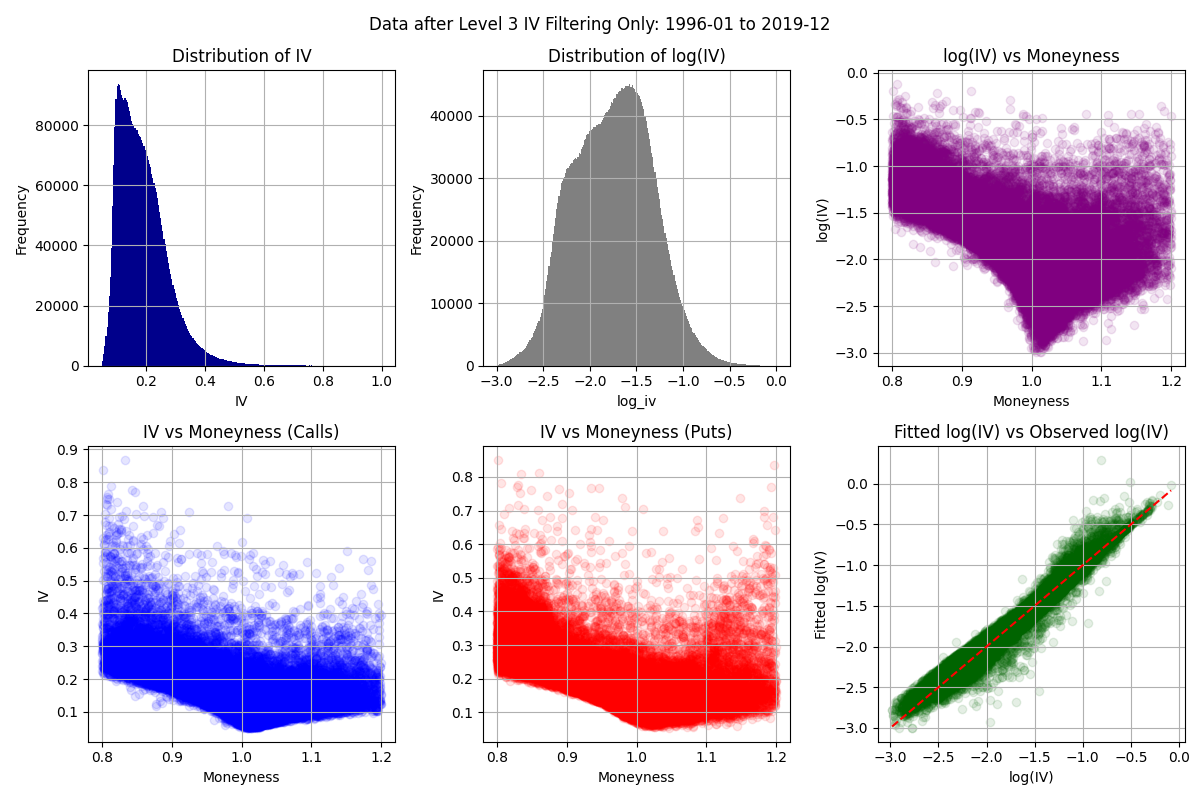
\includegraphics[width=\linewidth,height=0.666\linewidth]{../docs_src/L3_IV_1996-01_2019-12_iv.png}
  \caption{SPX options remaining after the Level 3 Implied Volatility filter (only).}
  \label{fig:l3_iv_only_spx_options_data}
\end{figure}


\begin{figure}[H]
  \centering
  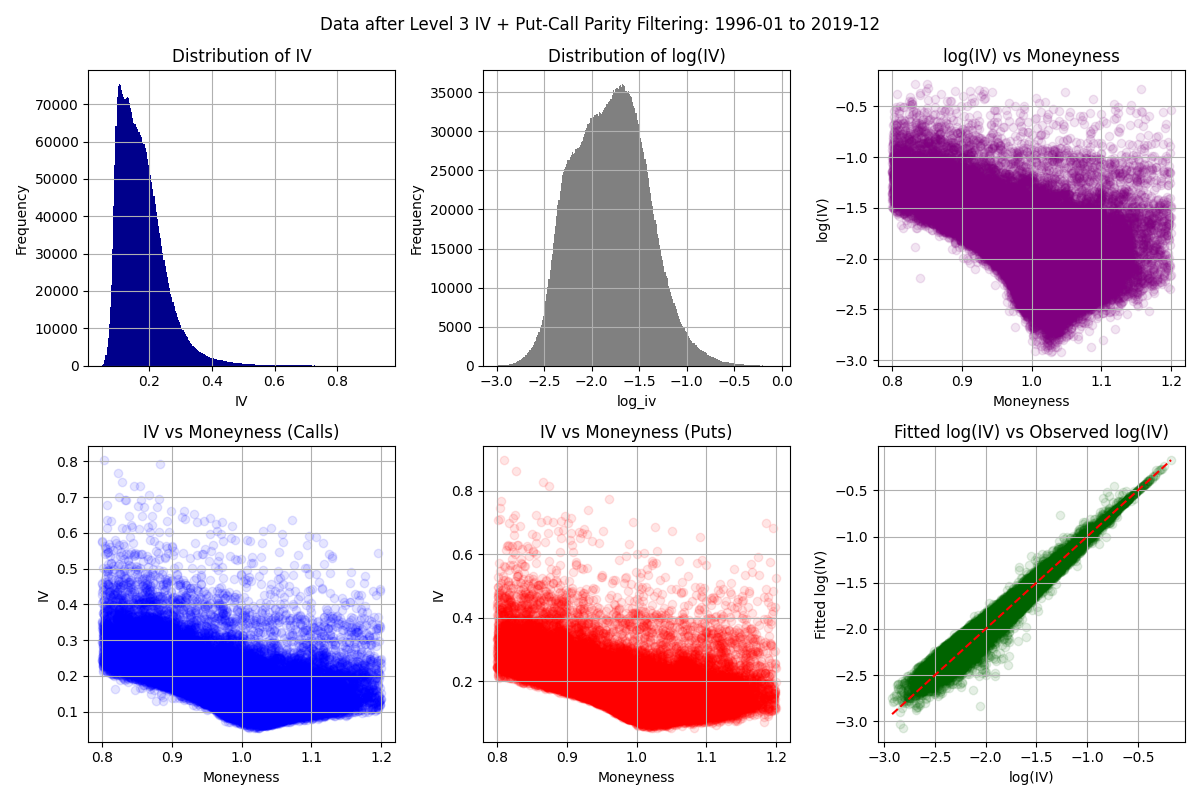
\includegraphics[width=\linewidth,height=0.666\linewidth]{../docs_src/L3_IV_PCP_1996-01_2019-12_iv.png}
  \caption{SPX options remaining after the Level 3 Implied Volatility and Put-Call Parity filters. Note how we observe the emergence of a volatility smile after the application of these filters.}
  \label{fig:l3_iv_pcp_spx_options_data}
\end{figure}


\subsection{Phase 1b: Portfolio Construction in \citet{Constantinides2013}}
\subsubsection{Construction of Monthly Leverage-Adjusted Portfolio Returns in CJS}

\paragraph{Process}
The construction of the 27 call and 27 put portfolios in CJS is a multi-step process, with the objective of developing portfolio returns series that are stationary and only moderately skewed. The discrete bucketing of moneyness and days to maturity leads to multiple candidate options for each portfolio on each trading day. These options are given weights according to a bivariate Gaussian weighting kernel in moneyness and maturity (bandwidths: 0.0125 in moneyness and 10 days to maturity).

Each portfolio's daily returns are initially calculated as simple arithmetic returns, assuming the option is bought and sold at its bid-ask midpoint at each rebalancing. The one-day arithmetic return is then converted to a leverage-adjusted return. This procedure is achieved by calculating the one-day return of a hypothetical portfolio with $\omega_{BSM}^{-1}$ dollars invested in the option, and $(1 - \omega_{BSM}^{-1})$ dollars invested in the risk-free rate, where $\omega_{BSM}$ is the Black-Scholes-Merton elasticity based on the implied volatility of the option.

\begin{align}
\omega_{\text{BSM, Call}} &= \frac{\partial C_{\text{BSM}}}{\partial S} \cdot \frac{S}{C_{\text{BSM}}} > 1 \\
\omega_{\text{BSM, Put}}  &= \frac{\partial P_{\text{BSM}}}{\partial S} \cdot \frac{S}{P_{\text{BSM}}} < -1
\end{align}

Each leverage-adjusted call portfolio comprises a long position in a fraction of a call, and some investment in the risk-free rate.

Each leverage-adjusted put portfolio comprises a short position in a fraction of a put, and more than 100\% investment in the risk-free rate.

\paragraph{Option Portfolio Construction Process}


Below, we formalize the CJS portfolio construction process for a single trading day $t$ and a set of candidate call or put options. Each portfolio is defined by option type (call or put), target moneyness (specifically $0.90$, $0.925$, $0.95$, $0.975$, $1.00$, $1.025$, $1.05$, $1.075$, $1.10$), and target maturity (specifically $30$, $60$, or $90$ days). On any given day, available options rarely match the targets exactly; instead, multiple candidate options may be close in moneyness and maturity. Each candidate option has its own price and sensitivity to the underlying index.

To aggregate these candidates, CJS applies a Gaussian kernel in moneyness and maturity, assigning weights to each option based on proximity to the targets. The kernel-weighted average price is used as the portfolio's option component. Portfolio returns are leverage-adjusted using Black-Scholes-Merton elasticity to standardize sensitivity across moneyness levels.

The daily portfolio return from $t$ to $t+1$ is computed as the kernel-weighted average return of the candidate options, using weights from day $t$. This approach ensures that each portfolio reflects the closest available options to the target characteristics, with appropriate adjustment for leverage and sensitivity.

\subsubsection{1. Gaussian Kernel Weighting}

Let:
\begin{itemize}
  \item $m_{i}$ = moneyness of option $i$
  \item $\tau_{i}$ = days to maturity of option $i$
  \item $k_{s}$ = target moneyness
  \item $\tau$ = target maturity
  \item $h_{m}$, $h_{\tau}$ = bandwidths for moneyness and maturity
  \item $d_{i}^2 = \left( \frac{m_{i} - k_{s}}{h_{m}} \right)^2 + \left( \frac{\tau_{i} - \tau}{h_{\tau}} \right)^2$
\end{itemize}

Then the unnormalized Gaussian weight for option $i$ is:
\[
w_{i}^* = \exp\left( -\frac{1}{2} d_{i}^2 \right)
\]

The normalized kernel weight:
\[
w_{i} = \frac{w_{i}^*}{\sum_j w_j^*}
\]

\subsubsection{2. Option Elasticity}

Let:
\begin{itemize}
  \item $S_{t}$ = underlying index level at time $t$
  \item $P_{i}$ = price of option $i$
  \item $\Delta_{i}$ = option delta
\end{itemize}

Then:
\[
\varepsilon_{i} = \frac{S_t \cdot \Delta_{i}}{P_{i}}
\]

\subsubsection{3. Arithmetic Return of Option $i$}

Let:
\begin{itemize}
  \item $P_{i,t-1}$ = price of option $i$ at time $t-1$
  \item $P_{i,t}$ = price of option $i$ at time $t$
\end{itemize}

Then:
\[
r_{i} = \frac{P_{i,t} - P_{i,t-1}}{P_{i,t-1}}
\]

\subsubsection{4. Leverage-Adjusted Portfolio Construction}

Let:
\begin{itemize}
  \item $r_{f}$ = risk-free rate on day $t$
\end{itemize}

The leverage-adjusted return of the call portfolio is:
\[
R_t^{call} = \sum_{i} w_{i} \cdot \frac{1}{\varepsilon_{i}} \cdot r_{i} + \left(1 - \sum_{i} w_{i} \cdot \frac{1}{\varepsilon_{i}} \right) \cdot r_f
\]

The leverage-adjusted return of the put portfolio is:
\[
R_t^{put} = -\sum_{i} w_{i} \cdot \frac{1}{\varepsilon_{i}} \cdot r_{i} + \left(1 + \sum_{i} w_{i} \cdot \frac{1}{\varepsilon_{i}} \right) \cdot r_f
\]



\subsubsection{5. Handling Missing Data (NaN Filling)}

CJS implement a multi-step process to address options with missing prices, as detailed in Section 1.3 ``Portfolio Formation'' of their paper. We reserve the implementation of this NaN-filling procedure for a future version of this dataset. For the current version, we compound the daily portfolio returns into monthly returns, which matches the final form of the data utilized in the paper.


\subsection{Phase 2: Returns Series Transformation in \citet{He2017}}
\subsubsection{Construction of 18 Portfolio Return Series in HKM}

\citet{He2017} reduce the 54 portfolios constructed in \citet{Constantinides2013} to 18 portfolios by taking an equal-weight average across the three maturities (30, 60, 90 days) for all CJS portfolios with the same moneyness. We implement that procedure to obtain the final return series for the FTSFR.

Let \( R_{m,j,t} \) be the return for moneyness \( m \), maturity \( j \), at time \( t \).
The HKM portfolio return for moneyness \( m \) at time \( t \) is:
\[
R_{m,t}^{\mathrm{HKM}} = \frac{1}{3} \sum_{j=1}^{3} R_{m,j,t}
\]
For each moneyness group, the HKM portfolio return is the simple average of the three corresponding CJS portfolio returns (one for each maturity) at each time point.

This averaging is done separately for calls and puts, resulting in 9 call portfolios and 9 put portfolios (total 18 portfolios).



\subsubsection{Portfolio Returns Analysis}

The objective of the data filtration process was to construct portfolios whose returns are approximately normal and only moderately skewed. We analyzed the distributional properties of the 54 CJS portfolios and the 18 HKM portfolios using standard statistical tests and summary statistics.

\paragraph{Statistical Normality Tests}
To assess the normality of portfolio returns, we applied several standard tests:
\begin{itemize}
  \item \textbf{Shapiro-Wilk Test:} Tests the null hypothesis that the data are drawn from a normal distribution. The test statistic is
  \[
  W = \frac{\left( \sum_{i=1}^n a_i x_{(i)} \right)^2}{\sum_{i=1}^n (x_i - \bar{x})^2}
  \]
  where $x_{(i)}$ are ordered sample values and $a_i$ are constants.
  \item \textbf{Jarque-Bera Test:} Tests whether sample skewness and kurtosis match a normal distribution. The test statistic is
  \[
  JB = \frac{n}{6} \left( S^2 + \frac{(K-3)^2}{4} \right)
  \]
  where $S$ is sample skewness and $K$ is sample kurtosis.
  \item \textbf{D'Agostino and Pearson's Normality Test (Normaltest):} Combines skewness and kurtosis to test for normality.
\end{itemize}
Low $p$-values (typically $<0.05$) indicate rejection of normality.

\paragraph{Summary Statistics}
Table~\ref{tab:portfolio_stats} presents descriptive statistics for the returns of the CJS and HKM portfolios. The statistics include count, mean, standard deviation, minimum, 25th percentile, median, 75th percentile, and maximum, following the convention of \texttt{pd.DataFrame.describe()}.

\begin{table}[H]
  \centering
  \caption{Descriptive Statistics of Portfolio Returns}
  \label{tab:portfolio_stats}
  \begin{tabular}{lcc}
    \toprule
    \textbf{Statistic} & \textbf{CJS Portfolios} & \textbf{HKM Portfolios} \\
    \midrule
    Count   & 54                          & 18                          \\
    Mean    & 1.64 (skew), 14.5 (kurtosis)  & 1.87 (skew), 16.8 (kurtosis) \\
    Std     & 2.26 (skew), 23.8 (kurtosis)  & 2.64 (skew), 30.3 (kurtosis) \\
    Min     & -0.91 (skew), 0.7 (kurtosis)  & -0.91 (skew), 0.7 (kurtosis) \\
    25\%    & 0.12 (skew), 2.1 (kurtosis)   & 0.12 (skew), 2.1 (kurtosis) \\
    \rowcolor{blue!20}
    Median  & 0.77 (skew), 4.6 (kurtosis)   & 0.78 (skew), 3.1 (kurtosis) \\
    75\%    & 2.41 (skew), 12.3 (kurtosis)  & 2.41 (skew), 12.3 (kurtosis) \\
    Max     & 11.1 (skew), 152.7 (kurtosis) & 9.8 (skew), 129.3 (kurtosis) \\
    \bottomrule
  \end{tabular}
\end{table}

\textbf{Note:} We did not implement the NaN-filling logic described in the original CJS paper. As a result, missing data may affect the distributional properties of the portfolio returns, and these results and conclusions may change in future versions once NaN handling is incorporated.

\paragraph{Results for CJS Portfolios}

Nearly all CJS portfolios reject normality based on the Shapiro-Wilk, Jarque-Bera, and Normaltest $p$-values, which are close to zero. The mean skewness is 1.64 and the median is 0.77, indicating distributions are generally right-skewed with long right tails. The mean kurtosis is 14.5 and the median is 4.6, suggesting many portfolios are leptokurtic (fat-tailed), with some experiencing rare but large return shocks. However, the median skewness and kurtosis are much closer to the normal values (skewness $=0$, kurtosis $=3$), implying that most portfolios are only moderately skewed and not excessively heavy-tailed. These results confirm that the filtration and leverage-adjustment procedures substantially mitigate extreme non-normality, achieving the authors' objective of constructing portfolios with returns that are approximately normal and only moderately skewed.

\paragraph{Results for HKM Portfolios}
Most HKM portfolios also reject normality, although a few have higher $p$-values and may plausibly be normal. The mean skewness is 1.87 and the median is 0.78, again showing generally positive skewness. The mean kurtosis is 16.8 and the median is 3.1, which is very close to the normal value of 3. This suggests that, while some portfolios have extreme outliers, the median HKM portfolio is only moderately skewed and has kurtosis similar to a normal distribution. These findings further validate that the aggregation and transformation steps in HKM produce portfolio returns with moderate skewness and near-normal kurtosis.

\paragraph{Overall Findings}
In summary, the data filtration and portfolio construction procedures yield return series that are not perfectly normal, but the median portfolio for both CJS and HKM is much closer to normal and only moderately skewed. This demonstrates that the authors' objectives were largely met: the median portfolio is well-suited for empirical asset pricing tests that assume approximate normality, even though some portfolios remain highly non-normal due to outliers. The successful replication of these distributional properties confirms the effectiveness of the canonical cleaning and construction methods.

\bibliographystyle{jpe}
\bibliography{bibliography}

\end{document}